\indent\indent In the \textit{Masks} menu, you'll find the \textit{Mask Images} feature. This option provides an easy way to remove images from your analysis. Select the images that you want to mask in your analysis to hide them from the analysis.\\

\begin{figure}[!h]
   \centering
   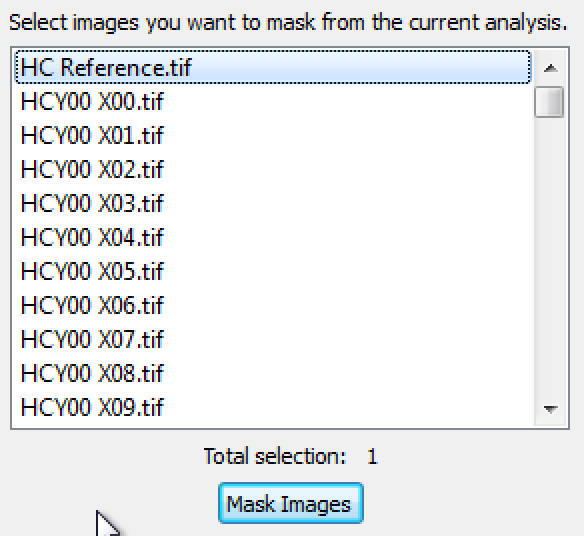
\includegraphics[scale=.6]{mask_images}
   \caption{Mask Images - Select images to hide}
\end{figure}

\newline
\indent When a mask is applied, the previous state of the analysis is automatically saved in the analysis folder.\\
On start-up, the software will load the last mask version by default. If you made a mistake or want to bring back your data, you can open a previous version by using the \text{Open Mask/Version} option in the \textit{File} menu.\\
\newline
\indent Please keep in mind that when a mask is applied, the data is only hidden and not modified. An older version can always be loaded.
